\documentclass{article}
\usepackage{hyperref}
\usepackage{graphicx} % Required for inserting images
\usepackage{xcolor}

\title{MapReduce}
\author{Mark Doughten [md1875], Abhilash Nambissan [ajn125], Rishita Mane [rm1848]}
\date{April 5, 2025}

\begin{document}

\maketitle
\section{Project Specification}

This report outlines our project plan for implementing MapReduce with GPU integration for handling large workloads.

\subsection{Goal}
At the end of the semester, the team wants to demonstrate that combining MapReduce and a GPU is beneficial and reduce the runtime for certain operations like counting. We aim to design a system that can perform distributed processing of compute jobs, by splitting the jobs into sub-tasks, and distributing sub-tasks across available CPUs and GPUs.

\subsection{Description}
This builds on the MapReduce framework designed at Google for clustering commodity hardware \cite{mapreduce}. Since then, we have seen the increase in need for more computing power for answering queries and training machine learning models. We feel that creating a framework that combines MapReduce and GPU will improved system design in the future and leverage both commodity hardware and advanced chips. 

\subsection{Outline}
The technical requirements are using CUDA which is the programming language designed specifically for operating on a NVIDIA GPU. That is combined with the technical details for MapReduce that are outlined in the paper \cite{mapreduce} and shown in Figure 1. 

\begin{figure}[ht]
    \centering
    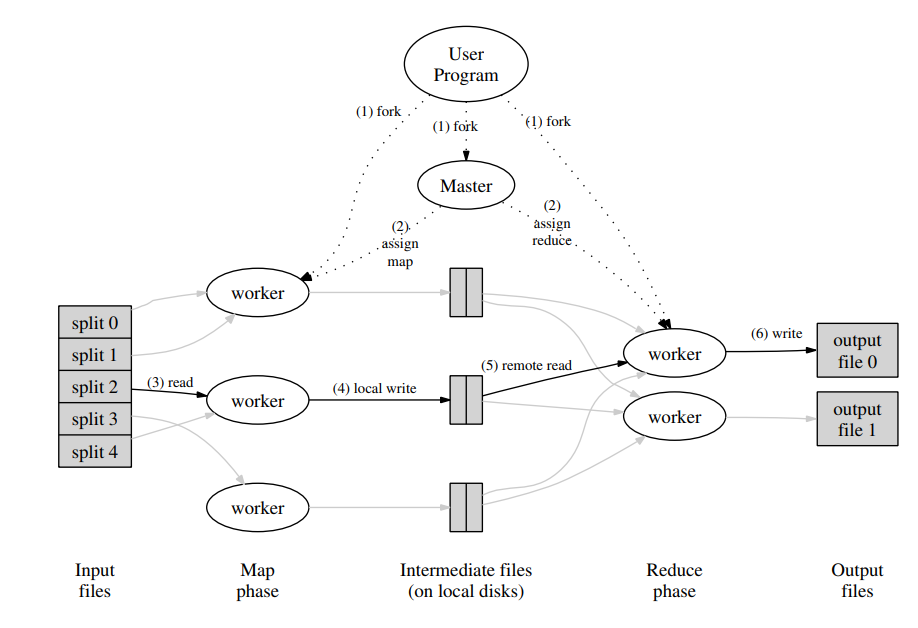
\includegraphics[width=1\linewidth]{./images/mapreduce.png}
    \caption{MapReduce \cite{mapreduce}}
    \label{fig:chroot}
\end{figure}

The combination of the two will require managing the load between the CPU and GPU since the data is exchanged between the two processors. That part will require optimization and an appropriate split.

\subsection{Measurements}
The team is going to measure the performance of various workloads on the system for measuring the overall effectiveness. The measurements will show the difference between running MapReduce on a CPU and then a CPU and a GPU. The measurements should challenge the hypothesis that combining MapReduce and a GPU is valuable and reducing processing time. We will measure various metrics such as throughput of the system in terms of operations per second, per operation latency, and total runtime for the entire map-reduce job.

\subsection{Risk}
The risk is getting the hardware required for completing this project since GPUs are in demand and CUDA is a proprietary language with limited capabilities. The experiment relies heavily on the configuration between MapReduce and NVIDIA GPU. 

\begin{thebibliography}{}
\raggedright

\bibitem{mapreduce}
MapReduce.
\href{https://dl.acm.org/doi/10.1145/1327452.1327492}{https://dl.acm.org/doi/10.1145/1327452.1327492}

\end{thebibliography}
\end{document}
